\section{lg\-Note Class Reference}
\label{classlgNote}\index{lgNote@{lgNote}}
A {\bf lg\-Event} with additional pitch info.  


{\tt \#include $<$lgnote.h$>$}

Inheritance diagram for lg\-Note::\begin{figure}[H]
\begin{center}
\leavevmode
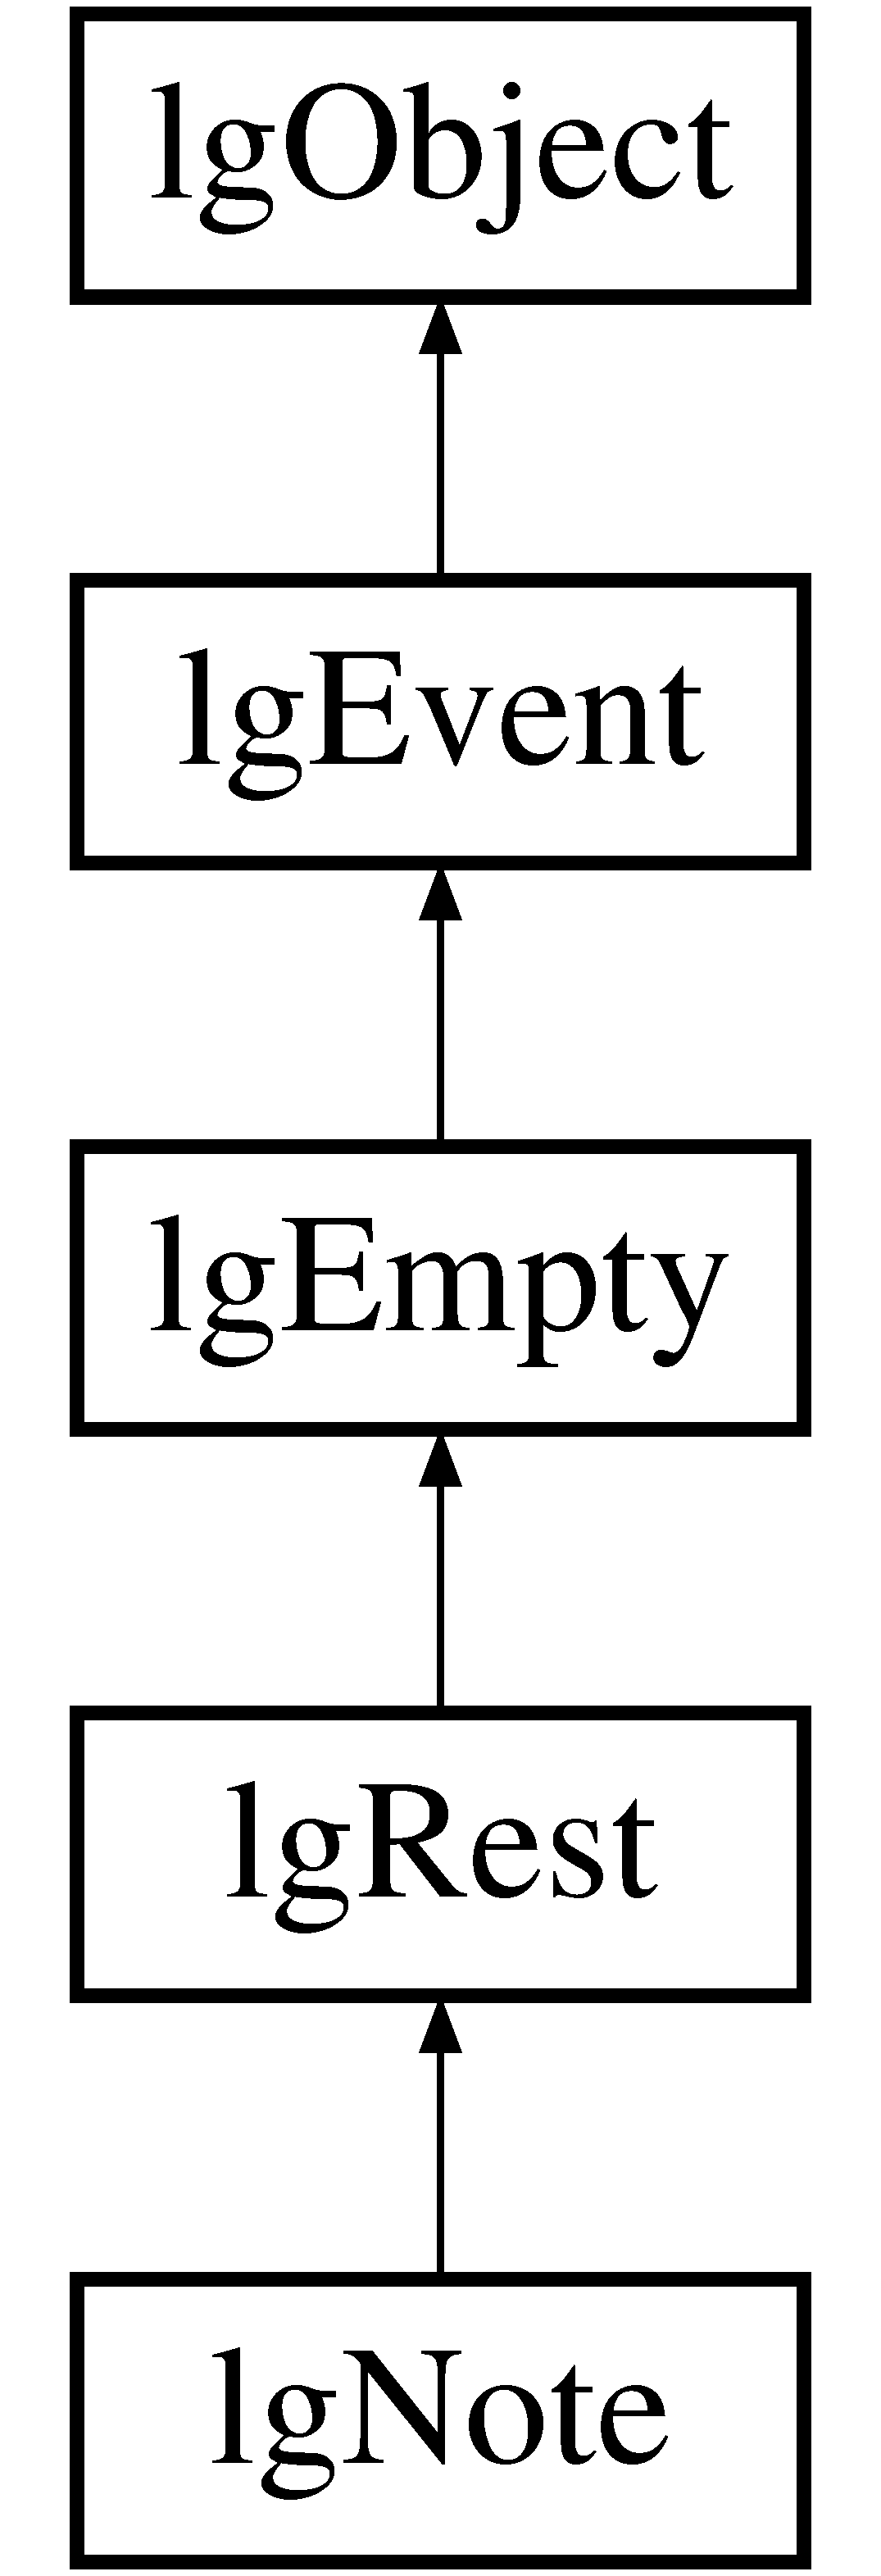
\includegraphics[height=5cm]{classlgNote}
\end{center}
\end{figure}
\subsection*{Public Member Functions}
\begin{CompactItemize}
\item 
virtual string {\bf to\-String} ({\bf lg\-Voice} $\ast$calling\-Seq=NULL)
\begin{CompactList}\small\item\em pitch accidentals octave $\ast$ duration \item\end{CompactList}\item 
int {\bf octave} (void)
\begin{CompactList}\small\item\em -oo...+oo, 0 == c' \item\end{CompactList}\item 
void {\bf set\-Octave} (int i)
\begin{CompactList}\small\item\em -oo...+oo, 0 == c' \item\end{CompactList}\item 
int {\bf pitch\-Class} (void)
\begin{CompactList}\small\item\em 0...11 = c,cis, ... b \item\end{CompactList}\item 
void {\bf set\-Pitch\-Class} (int i)
\begin{CompactList}\small\item\em 0...11 = c,cis, ... b \item\end{CompactList}\item 
int {\bf accidentals} (void)
\begin{CompactList}\small\item\em -oo..+oo \item\end{CompactList}\item 
void {\bf set\-Accidentals} (int i)
\begin{CompactList}\small\item\em -oo..+oo \item\end{CompactList}\item 
{\bf lg\-Note} (int pc, int oct, int acc, long int dur\-Num, long int dur\-Denom, int cdots, long int pos\-Num, long int pos\-Denom)
\item 
string {\bf pitch} (void)
\begin{CompactList}\small\item\em pitch as string \char`\"{}c\char`\"{}, \char`\"{}c\#\char`\"{}, \char`\"{}gis\char`\"{}, \char`\"{}g\#\char`\"{}, ... \item\end{CompactList}\end{CompactItemize}
\subsection*{Private Attributes}
\begin{CompactItemize}
\item 
int {\bf pitch\-Class\-I}
\begin{CompactList}\small\item\em 0..11 = c,cis,...,b \item\end{CompactList}\item 
int {\bf octave\-I}
\begin{CompactList}\small\item\em -oo .. +oo, 0 = c' \item\end{CompactList}\item 
int {\bf accidentals\-I}
\begin{CompactList}\small\item\em -oo .. +oo \item\end{CompactList}\end{CompactItemize}


\subsection{Detailed Description}
A {\bf lg\-Event} with additional pitch info. 



\subsection{Constructor \& Destructor Documentation}
\index{lgNote@{lg\-Note}!lgNote@{lgNote}}
\index{lgNote@{lgNote}!lgNote@{lg\-Note}}
\subsubsection{\setlength{\rightskip}{0pt plus 5cm}lg\-Note::lg\-Note (int {\em pc}, int {\em oct}, int {\em acc}, long int {\em dur\-Num}, long int {\em dur\-Denom}, int {\em cdots}, long int {\em pos\-Num}, long int {\em pos\-Denom})}\label{classlgNote_a7}


\begin{Desc}
\item[Parameters: ]\par
\begin{description}
\item[{\em 
pc}]pitchclass 0..11 \item[{\em 
oct}]octave -oo..+oo, 0 = c' \item[{\em 
acc}]\# of accidentals -oo .. +oo \item[{\em 
dur\-Num}]duration numerator \item[{\em 
dur\-Denom}]duration denominator \item[{\em 
cdots}]\# of dots \item[{\em 
pos\-Num}]position numerator \item[{\em 
pos\-Denom}]position denominator \end{description}
\end{Desc}


\subsection{Member Function Documentation}
\index{lgNote@{lg\-Note}!accidentals@{accidentals}}
\index{accidentals@{accidentals}!lgNote@{lg\-Note}}
\subsubsection{\setlength{\rightskip}{0pt plus 5cm}int lg\-Note::accidentals (void)\hspace{0.3cm}{\tt  [inline]}}\label{classlgNote_a5}


-oo..+oo 

\index{lgNote@{lg\-Note}!octave@{octave}}
\index{octave@{octave}!lgNote@{lg\-Note}}
\subsubsection{\setlength{\rightskip}{0pt plus 5cm}int lg\-Note::octave (void)}\label{classlgNote_a1}


-oo...+oo, 0 == c' 

\index{lgNote@{lg\-Note}!pitch@{pitch}}
\index{pitch@{pitch}!lgNote@{lg\-Note}}
\subsubsection{\setlength{\rightskip}{0pt plus 5cm}string lg\-Note::pitch (void)}\label{classlgNote_a8}


pitch as string \char`\"{}c\char`\"{}, \char`\"{}c\#\char`\"{}, \char`\"{}gis\char`\"{}, \char`\"{}g\#\char`\"{}, ... 

copy pitch class \index{lgNote@{lg\-Note}!pitchClass@{pitchClass}}
\index{pitchClass@{pitchClass}!lgNote@{lg\-Note}}
\subsubsection{\setlength{\rightskip}{0pt plus 5cm}int lg\-Note::pitch\-Class (void)}\label{classlgNote_a3}


0...11 = c,cis, ... b 

\index{lgNote@{lg\-Note}!setAccidentals@{setAccidentals}}
\index{setAccidentals@{setAccidentals}!lgNote@{lg\-Note}}
\subsubsection{\setlength{\rightskip}{0pt plus 5cm}void lg\-Note::set\-Accidentals (int {\em i})\hspace{0.3cm}{\tt  [inline]}}\label{classlgNote_a6}


-oo..+oo 

\index{lgNote@{lg\-Note}!setOctave@{setOctave}}
\index{setOctave@{setOctave}!lgNote@{lg\-Note}}
\subsubsection{\setlength{\rightskip}{0pt plus 5cm}void lg\-Note::set\-Octave (int {\em i})\hspace{0.3cm}{\tt  [inline]}}\label{classlgNote_a2}


-oo...+oo, 0 == c' 

\index{lgNote@{lg\-Note}!setPitchClass@{setPitchClass}}
\index{setPitchClass@{setPitchClass}!lgNote@{lg\-Note}}
\subsubsection{\setlength{\rightskip}{0pt plus 5cm}void lg\-Note::set\-Pitch\-Class (int {\em i})\hspace{0.3cm}{\tt  [inline]}}\label{classlgNote_a4}


0...11 = c,cis, ... b 

\index{lgNote@{lg\-Note}!toString@{toString}}
\index{toString@{toString}!lgNote@{lg\-Note}}
\subsubsection{\setlength{\rightskip}{0pt plus 5cm}string lg\-Note::to\-String ({\bf lg\-Voice} $\ast$ {\em calling\-Seq} = NULL)\hspace{0.3cm}{\tt  [virtual]}}\label{classlgNote_a0}


pitch accidentals octave $\ast$ duration 



Reimplemented from {\bf lg\-Rest} {\rm (p.\,\pageref{classlgRest_a0})}.

\subsection{Member Data Documentation}
\index{lgNote@{lg\-Note}!accidentalsI@{accidentalsI}}
\index{accidentalsI@{accidentalsI}!lgNote@{lg\-Note}}
\subsubsection{\setlength{\rightskip}{0pt plus 5cm}int {\bf lg\-Note::accidentals\-I}\hspace{0.3cm}{\tt  [private]}}\label{classlgNote_r2}


-oo .. +oo 

\index{lgNote@{lg\-Note}!octaveI@{octaveI}}
\index{octaveI@{octaveI}!lgNote@{lg\-Note}}
\subsubsection{\setlength{\rightskip}{0pt plus 5cm}int {\bf lg\-Note::octave\-I}\hspace{0.3cm}{\tt  [private]}}\label{classlgNote_r1}


-oo .. +oo, 0 = c' 

\index{lgNote@{lg\-Note}!pitchClassI@{pitchClassI}}
\index{pitchClassI@{pitchClassI}!lgNote@{lg\-Note}}
\subsubsection{\setlength{\rightskip}{0pt plus 5cm}int {\bf lg\-Note::pitch\-Class\-I}\hspace{0.3cm}{\tt  [private]}}\label{classlgNote_r0}


0..11 = c,cis,...,b 



The documentation for this class was generated from the following files:\begin{CompactItemize}
\item 
{\bf lgnote.h}\item 
{\bf lgnote.cpp}\end{CompactItemize}
